\documentclass[11pt]{article}
\usepackage[margin=1.2in]{geometry}
\usepackage{graphicx}
\usepackage{fancyhdr}
\usepackage{nopageno}%removes number on titlepage
\usepackage[parfill]{parskip}
%\usepackage{subfig}
\usepackage{multirow}
\usepackage{caption}
\usepackage{subcaption}

\begin{document}
% Cover page
\author{Chelsey Legacy, Lindong Zhou, Evan Pete Walsh\footnote{Statistics graduate students at Iowa State University of Science and Technology}}
\title{STAT 579 Final Project}
\maketitle

\begin{abstract}
Analysis of the Yelp Academic Dataset.
\end{abstract}

\newpage

\tableofcontents

\newpage

\pagenumbering{arabic}%starts numbering at "1"
\pagestyle{fancy}
\fancyhead[L]{Iowa State University}
\rhead{\thepage}
\rfoot{\today}
\cfoot{}%removes default page number at bottom center


\subsection{Delivery vs. Takeout}

\begin{figure}[h!]
  \caption{Plot of if a restaurant does takeout orders colored by if they do deliveries and faceted by the type of food the restaurant serves.}
  \centering
  \label{takeout}
    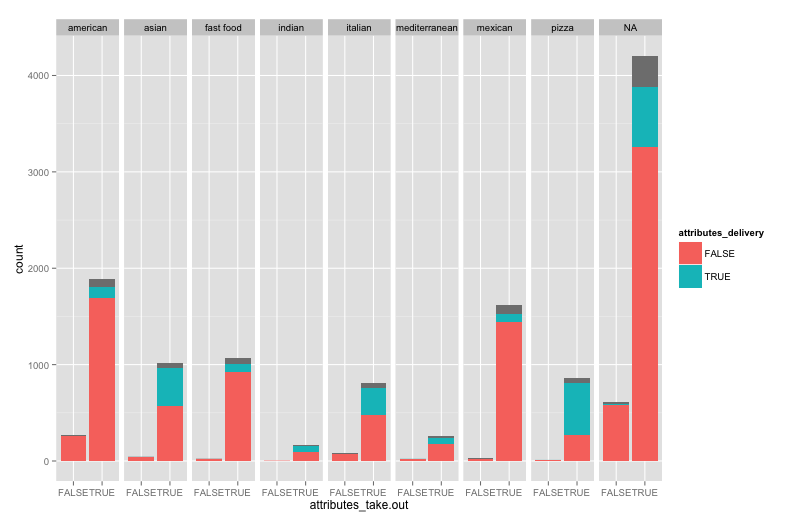
\includegraphics[width=0.9\textwidth]{Figures/takeoutdelivery.png}
\end{figure}
Now we know have gained some insight into restaurants' price and reservation style, but what about when you do not want to go eat at the restaurant? Some days there is little time for cooking, so people commonly call out for delivery or take out.  But what types of food are most likely to have delivery or takeout?  In other words, if we are ordering out, what is it likely we will be able to have delivered to us and what can we pick up on our way home? In 
Figure~\ref{takeout} we can see that the food types that most likely have delivery are those that serve pizza, Asian, or possibly Italian.  Most likely you will not be able to find an American or fast food place that delivers.  This could be due to the fact that some of these foods do not stay good if they sit too long.  Foods like pizza and rice are fine to sit for a while,  are easy to keep warm and fresh tasting, and can also be easily reheated. Thus, these are qualities that make them good options for delivery.  However, American food, or fast food like burgers and fries are not good if they sit too long, and do not reheat to the quality they were when they left the restaurant.  Thus, there are fewer, if any of these places that offer delivery.

We can see in more detail in Figure~\ref{takeout} that restaurants of all types are much more likely to offer takeout than delivery to customers.  We can also see that the restaurant is more likely to offer delivery if they offer a takeout option.  Restaurants of all types may be more inclined to offer delivery than takeout for a number of reasons.  They could only have a limited number of people working and do not want to spare any or pay extra people to deliver the food.  Delivery also means transportation costs for the business, and as discussed above it means more time for the food to decrease in quality while a driver makes several deliveries.  However, takeout is a great option for restaurants, because they get to sell more food, without have to seat as many people in the restaurant.  Takeout also reduces the responsibility of the quality of the food once it arrives at its destination.  If it took the customer a long time to get home and the food is not as good as it once was, this is not the restaurant's fault.  



\section{Bars}

The Business dataset contains a lot of information that can be used to analyze the relationship between different aspects of bar culture.  In order to analyze the bars available in the dataset, the data was subset to get rid of any businesses that did not have a full bar.  Looking at only the businesses with a full bar gives us insight into locations that serve from a full bar such as clubs, hotels, select restaurants, lounges, bowling alleys, and other various entertainment locations.  Through analyzing this data we can explore what types of food are served at bars (if any), if lower ratings indicate a bar could shut down, and the type of activities that might take place at a given bar.

\subsection{Food}

\begin{figure}[h!]
  \caption{Plot of the number of stars a restaurant received filled with the type of food served at the bar.}
  \centering
  \label{food}
    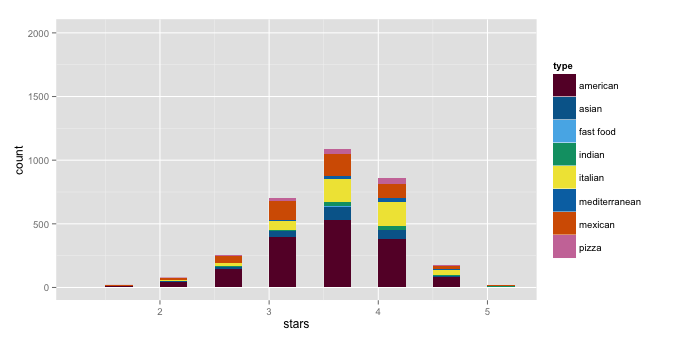
\includegraphics[width=0.75\textwidth]{Figures/Food_bars.png}
\end{figure}

Though not all bars serve food, many bars in restaurants do which begs the question; what is the most common food served in bars?  In order to investigate this question a qplot of the number of starts given to each bar filled with a count of the food types for each different rating will give us this information and more.  This data revealed, unsurprisingly, that the most common food served in American bars is American food (burgers, fries, etc). Through further analysis it is determined that 50$\%$ of the bars that serve food served primarily American style food.  We can see that the majority of each bar of star, no matter what the rating, is colored for American food.  However, looking more closely at the graph we can see that there is some unexpected information.  From Figure~\ref{food} we can see that there are a wide number of food options for people looking for full bars.  Along with American, Italian and Mexican are also abundant options making up 16$\%$ and 16.7$\%$ respectively.  Another piece of information we can infer from this graphic is that along with the plot of the stars a bar receives being a normal distribution, there also is a consistency in the number of each type of food being represented at each level of stars a bar receives.  Thus, we can see there is no preference for food when looking for a certain quality bar. A bar is equally likely to serve American food whether it receives 1 star or 5 stars.  This could be further investigated through hypothesis testing for difference in proportions.

\subsection{Stars}
\begin{figure}[h!]
  \caption{Plot of the number of stars a bar received colored by whether or not they are open or closed}
  \centering
  \label{open}
    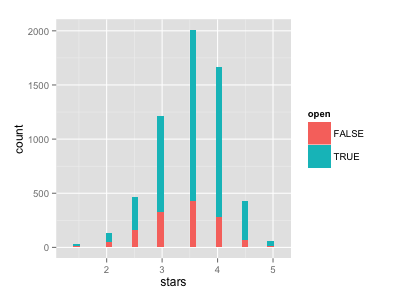
\includegraphics[width=0.5\textwidth]{Figures/barstatus.png}
\end{figure}
The purpose of yelp is to provide review of businesses for others in the community to take into consideration.  Since this dataset provides the number stars a bar receives and the status of the bar (open or closed) as of when the data was collected.  We decided to investigate the idea that possibly if the bar has lower ratings it has more of a chance of being closed.  However, if inspected closely looking at the extreme endpoints of the graph you can see it appears the percent of open restaurants at the 5 star level is higher than the percent of 1 star restaurants that are open. In order to look into this further we created several subsets of the data.  We created a subset of data for 2 stars(1 star had 0 observations), 3.5 stars (which is the median of the data), and 5 stars.  We then found the percent of open bars for each level.  We found that the 2 stars had 64.3$\%$ open, the 3.5 stars had 78.4$\%$ and 5 stars had 82.1$\%$ open.  As we can see the percentages of bars open increases as the number of stars the bar is rated increases.  Though we can make no assumptions of causation, this is still an interesting trend to consider for further more complex analysis.

\subsection{Popular Features}
\begin{figure}
\centering
\begin{subfigure}{.5\textwidth}
  \centering
  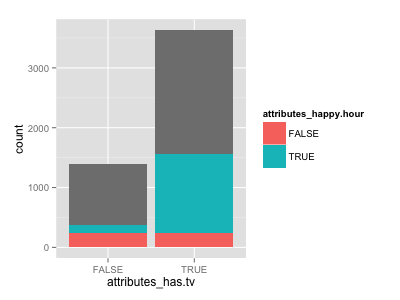
\includegraphics[width=0.75\linewidth]{Figures/tvhappyhour.png}
  \caption{Plot indicating whether or not the bar as a tv, colored by if it has happy hour specials}
  \label{happy}
\end{subfigure}%
\begin{subfigure}{.5\textwidth}
  \centering
  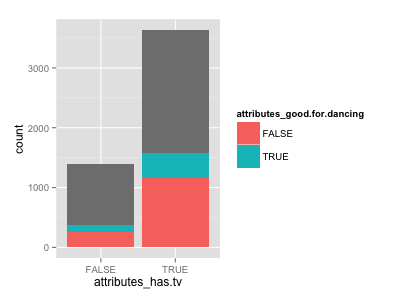
\includegraphics[width=0.75\linewidth]{Figures/tvdancing.png}
  \caption{Plot indicating whether or not the bar as a tv, colored by if it is good for dancing}
  \label{dance}
\end{subfigure}
\caption{}
\label{}
\end{figure}

\vspace{5mm}
Each bar in a community has its own unique features, special pricing promotions, or atmosphere.  Some bars are good for dancing, watching televisions broadcasting sports games, happy hour, or some are more quiet and laid back for just talking and relaxing with friends.  What are the relationships between these variables, if any?  We wanted to find characteristics for each of the  different atmospheres a bar may have: romantic, intimate, touristy, hipster, divey, classy, trendy, upscale, and casual.  However, it quickly became clear that there are not many bars in each of these categories.  Most bars are just classified as casual.  Thus, there wasn't much to investigate.



Next, we thought it would be interesting to look at features of bars with televisions.  Since, not all bars have televisions there must be certain characteristics for those that choose to have a television and those that do not.   In  Figure~\ref{happy} we can see that most bars that have a tv also have happy hour specials.  These are probably more causal places that people go after work to relax with coworkers and friends.  We can gain even more insight into the bars with tvs when we look at  Figure~\ref{dance}.  In this plot it is interestingly apparent that if a bar has a tv it is more likely that it is not good for dancing.  This again reinforces that the bars with televisions are more of a relaxed atmosphere to hang out and chat or watch sports.  Most likely a place like this would be an in inappropriate atmosphere for a group looking to go dancing.  Places people go dancing are more apt to be louder places people go later at night, when happy hour specials would be over and there would be no need for televisions while dancing.  



\section{Conclusion}

The Yelp Academic Dataset has provided us information on a variety of businesses including restaurants, bars, hotels, and shops.  We have used the abundance of data to find key relationships between the available variables and their respective businesses.  For example, we have found that reservations, price, noise level, takeout, delivery, and foremost service are key variables that provide interesting relationships for restaurant data.  We have also found that features such as food type, if a restaurant has a TV, or if it is good for dancing all provide insight into what type of atmosphere we will find at a bar.  When evaluating hotels and shopping we have found that popularity does not always reflect the quality of the service we will receive.  This data set has provided us with many insights into possible relationships between not only these variables, but also human culture and tendencies.  Though it is impossible to make solid conclusions about any of the relationships we have found based on our limited dataset, we have still come up with some interesting relationships and found even more questions about this topic that could be used for further research on the subject.





\end{document}